\documentclass{article}

\usepackage{arxiv}

\usepackage[utf8]{inputenc} % allow utf-8 input
\usepackage[T1]{fontenc}    % use 8-bit T1 fonts
\usepackage{lmodern}        % https://github.com/rstudio/rticles/issues/343
\usepackage{hyperref}       % hyperlinks
\usepackage{url}            % simple URL typesetting
\usepackage{booktabs}       % professional-quality tables
\usepackage{amsfonts}       % blackboard math symbols
\usepackage{nicefrac}       % compact symbols for 1/2, etc.
\usepackage{microtype}      % microtypography
\usepackage{graphicx}

\title{Machine Learning Methods for Modeling and Classification of
fashion MNIST}

\author{
    David Blumenstiel
   \\
    Department of Data Science and Information Systems \\
    CUNY School of Professional Studies \\
  NY, NY 1001 \\
  \texttt{\href{mailto:blumenstieldavid@gmail.com}{\nolinkurl{blumenstieldavid@gmail.com}}} \\
   \And
    Bonnie Cooper
   \\
    Department of Biological Sciences \\
    SUNY College of Optometry \\
  NY, NY 10036 \\
  \texttt{\href{mailto:bcooper@sunyopt.edu}{\nolinkurl{bcooper@sunyopt.edu}}} \\
   \And
    Robert Welk
   \\
    Department of Data Science and Information Systems \\
    CUNY School of Professional Studies \\
  NY, NY 1001 \\
  \texttt{\href{mailto:robert.j.welk@gmail.com}{\nolinkurl{robert.j.welk@gmail.com}}} \\
   \And
    Leo Yi
   \\
    Department of Data Science and Information Systems \\
    CUNY School of Professional Studies \\
  NY, NY 1001 \\
  \texttt{\href{mailto:leo.yi35@spsmail.cuny.edu}{\nolinkurl{leo.yi35@spsmail.cuny.edu}}} \\
  }

\usepackage{color}
\usepackage{fancyvrb}
\newcommand{\VerbBar}{|}
\newcommand{\VERB}{\Verb[commandchars=\\\{\}]}
\DefineVerbatimEnvironment{Highlighting}{Verbatim}{commandchars=\\\{\}}
% Add ',fontsize=\small' for more characters per line
\usepackage{framed}
\definecolor{shadecolor}{RGB}{248,248,248}
\newenvironment{Shaded}{\begin{snugshade}}{\end{snugshade}}
\newcommand{\AlertTok}[1]{\textcolor[rgb]{0.94,0.16,0.16}{#1}}
\newcommand{\AnnotationTok}[1]{\textcolor[rgb]{0.56,0.35,0.01}{\textbf{\textit{#1}}}}
\newcommand{\AttributeTok}[1]{\textcolor[rgb]{0.77,0.63,0.00}{#1}}
\newcommand{\BaseNTok}[1]{\textcolor[rgb]{0.00,0.00,0.81}{#1}}
\newcommand{\BuiltInTok}[1]{#1}
\newcommand{\CharTok}[1]{\textcolor[rgb]{0.31,0.60,0.02}{#1}}
\newcommand{\CommentTok}[1]{\textcolor[rgb]{0.56,0.35,0.01}{\textit{#1}}}
\newcommand{\CommentVarTok}[1]{\textcolor[rgb]{0.56,0.35,0.01}{\textbf{\textit{#1}}}}
\newcommand{\ConstantTok}[1]{\textcolor[rgb]{0.00,0.00,0.00}{#1}}
\newcommand{\ControlFlowTok}[1]{\textcolor[rgb]{0.13,0.29,0.53}{\textbf{#1}}}
\newcommand{\DataTypeTok}[1]{\textcolor[rgb]{0.13,0.29,0.53}{#1}}
\newcommand{\DecValTok}[1]{\textcolor[rgb]{0.00,0.00,0.81}{#1}}
\newcommand{\DocumentationTok}[1]{\textcolor[rgb]{0.56,0.35,0.01}{\textbf{\textit{#1}}}}
\newcommand{\ErrorTok}[1]{\textcolor[rgb]{0.64,0.00,0.00}{\textbf{#1}}}
\newcommand{\ExtensionTok}[1]{#1}
\newcommand{\FloatTok}[1]{\textcolor[rgb]{0.00,0.00,0.81}{#1}}
\newcommand{\FunctionTok}[1]{\textcolor[rgb]{0.00,0.00,0.00}{#1}}
\newcommand{\ImportTok}[1]{#1}
\newcommand{\InformationTok}[1]{\textcolor[rgb]{0.56,0.35,0.01}{\textbf{\textit{#1}}}}
\newcommand{\KeywordTok}[1]{\textcolor[rgb]{0.13,0.29,0.53}{\textbf{#1}}}
\newcommand{\NormalTok}[1]{#1}
\newcommand{\OperatorTok}[1]{\textcolor[rgb]{0.81,0.36,0.00}{\textbf{#1}}}
\newcommand{\OtherTok}[1]{\textcolor[rgb]{0.56,0.35,0.01}{#1}}
\newcommand{\PreprocessorTok}[1]{\textcolor[rgb]{0.56,0.35,0.01}{\textit{#1}}}
\newcommand{\RegionMarkerTok}[1]{#1}
\newcommand{\SpecialCharTok}[1]{\textcolor[rgb]{0.00,0.00,0.00}{#1}}
\newcommand{\SpecialStringTok}[1]{\textcolor[rgb]{0.31,0.60,0.02}{#1}}
\newcommand{\StringTok}[1]{\textcolor[rgb]{0.31,0.60,0.02}{#1}}
\newcommand{\VariableTok}[1]{\textcolor[rgb]{0.00,0.00,0.00}{#1}}
\newcommand{\VerbatimStringTok}[1]{\textcolor[rgb]{0.31,0.60,0.02}{#1}}
\newcommand{\WarningTok}[1]{\textcolor[rgb]{0.56,0.35,0.01}{\textbf{\textit{#1}}}}


% Pandoc citation processing
\newlength{\csllabelwidth}
\setlength{\csllabelwidth}{3em}
\newlength{\cslhangindent}
\setlength{\cslhangindent}{1.5em}
% for Pandoc 2.8 to 2.10.1
\newenvironment{cslreferences}%
  {}%
  {\par}
% For Pandoc 2.11+
\newenvironment{CSLReferences}[2] % #1 hanging-ident, #2 entry spacing
 {% don't indent paragraphs
  \setlength{\parindent}{0pt}
  % turn on hanging indent if param 1 is 1
  \ifodd #1 \everypar{\setlength{\hangindent}{\cslhangindent}}\ignorespaces\fi
  % set entry spacing
  \ifnum #2 > 0
  \setlength{\parskip}{#2\baselineskip}
  \fi
 }%
 {}
\usepackage{calc} % for calculating minipage widths
\newcommand{\CSLBlock}[1]{#1\hfill\break}
\newcommand{\CSLLeftMargin}[1]{\parbox[t]{\csllabelwidth}{#1}}
\newcommand{\CSLRightInline}[1]{\parbox[t]{\linewidth - \csllabelwidth}{#1}\break}
\newcommand{\CSLIndent}[1]{\hspace{\cslhangindent}#1}



\begin{document}
\maketitle

\def\tightlist{}


\begin{abstract}
Fashion MNIST is a clothing classification dataset that is popular for
deep learning and computer vision applications. In this report, we use
Fashion MNIST to apply multiple machine learning methods reviewed in
Data622: Machine Learning and Big Data, an elective course for the
Masters of Science in Data Science at CUNY School of Professional
Studies. We explore approaches to reduce the dimensionality of the data
by engineering new descriptive features and performing Principal
Components Analysis. We then follow this up with machine learning
methods for classification such as Support Vector Machine and a
Convolutional Neural Network. We find that
\end{abstract}

\keywords{
    fashion MNIST
   \and
    machine learning
   \and
    classification
  }

\hypertarget{introduction}{%
\section{Introduction}\label{introduction}}

Fashion MNIST is a clothing classification dataset that builds in
complexity in comparison to the classic MNIST dataset. MNIST is a
dataset of handwritten digits that has been a go-to dataset for
benchmarking various image processing and machine learning algorithms
(LeCun et al. 1998). Classification algorithms applied to MNIST
revolutionized the field of image processing in the 90s (Krizhevsky,
Hinton, and others 2009). However, contemporary machine learning methods
can achieve 97\% accuracy. Convolutional neural networks score as high
as 99.7\% accuracy. As a result, MNIST is now considered too easy and,
with \textasciitilde48000 MNIST related publications (Noever and Noever
2021), MNIST has also been used by the machine learning community
exhaustively. Fashion MNIST was developed as an alternative.

Fashion MNIST can serve as a direct drop-in replacement for MNIST.
Fashion MNIST and MNIST are both labeled data that share the same
dataset size: 60,000 training images and 10,000 test images.
Additionally, Fashion MNIST and MNIST images share the same dimensions
and structure: 10 distinct categories of grayscale images with 28x28
pixel size. Figure 1 depicts a sampling of several dozen example
Fashion-MNIST images. Due to the complexity and variety of the images,
Fashion MNIST is a more challenging dataset for machine learning
algorithms (Xiao, Rasul, and Vollgraf 2017).

\begin{figure}

{\centering 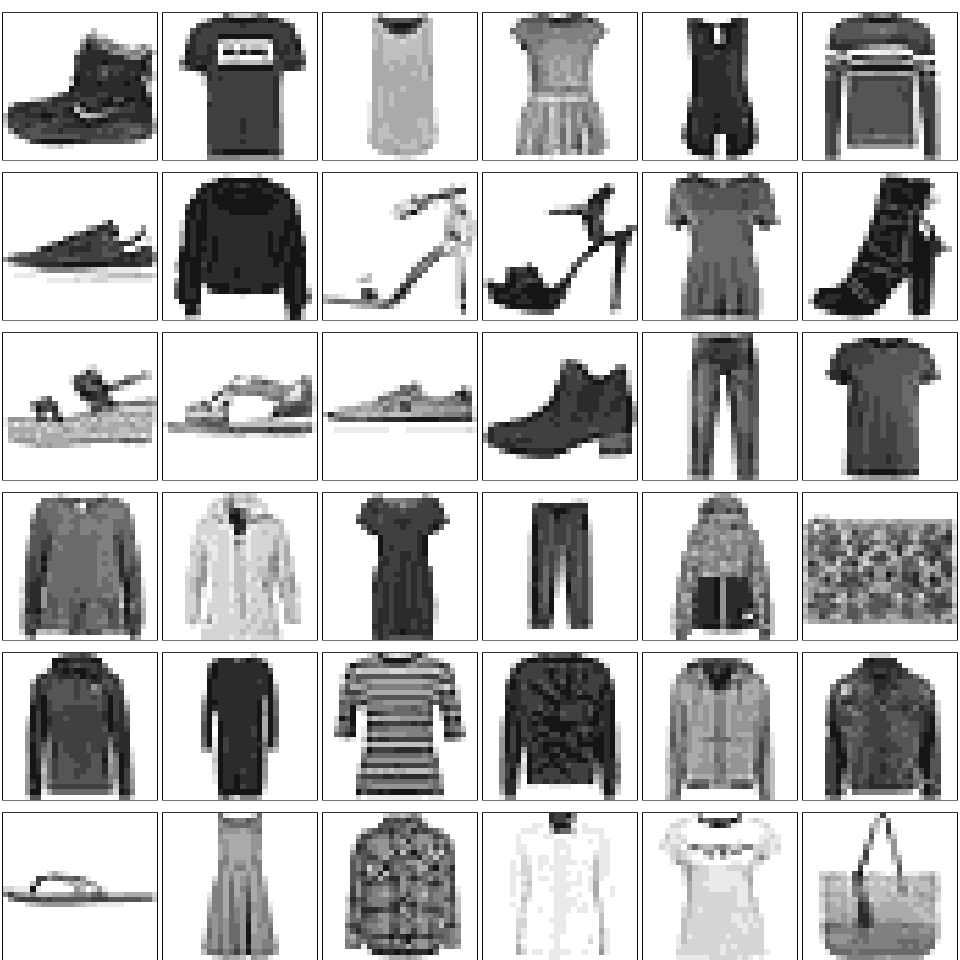
\includegraphics[width=0.6\linewidth]{/home/bonzilla/Documents/MSDS/Data622_group5_projects/FinalReport_Data622/exemplars} 

}

\caption{Exemplar Fashion-MNIST images. All image files are grayscale 28x28 images}\label{fig:unnamed-chunk-1}
\end{figure}

In this report we utilize Fashion MNIST to implement a variety of
machine learning approaches covered over the course of our studies in
Data622: Machine Learning and Big Data as part of the Masters of Data
Science program at CUNY School of Professional Studies. Our goal is to
optimize the classification of Fashion MNIST images using a variety of
machine learning algorithms. Here, we describe our approaches and
compare classification model performance.

With an image size of 28 x 28, Fashion MNIST images, in their raw form,
are high dimensional data with a total of 784 features. Additionally,
there is a relatively high degree of correlation between pixel values of
a given image. That is to say that, unless an pixel is at an object
border, a light pixel in a region of the image is very likely to be
situated next to light neighboring pixels, likewise for dark pixels. We
can assess this by observing the mean and standard deviation of the
pixel values across the dataset.

Figure 2 visualizes the mean (left) and standard deviations (right) of
the pixel values for the \texttt{train} dataset. For both plots, higher
intensity values are rendered as dark whereas low values are light. For
many of the pixels in the image, the mean values are intermediate (gray)
whereas the corresponding standard deviations are relatively high
(dark). These pixels make up most of the variance in the dataset.
However, we can see that there are two regions of pixels towards the
image center where the mean pixel value is high (dark) while the pixel
standard deviation is low (light). For these regions, the pixels have
consistently high pixel values. Towards the periphery of the image there
are pixels with both low mean values (light) and low standard deviation
(light). These pixels have consistently low values. The pixels with
either consistently low or high values are of low information content
and would not contribute much to models for image classification if used
as features. Therefore, we describe two methods for reducing the
dimensionality of the Fashion-MNIST dataset. Furthermore, this report
goes on to describe multiple different models developed from the
resulting reduced sets and evaluate the performances.

\begin{figure}

{\centering 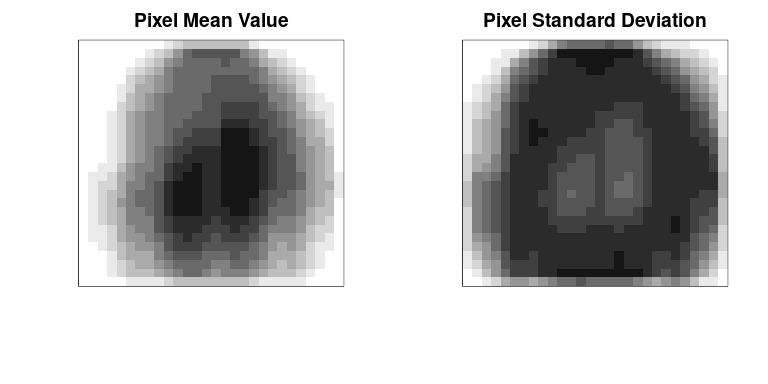
\includegraphics[width=0.9\linewidth]{/home/bonzilla/Documents/MSDS/Data622_group5_projects/FinalReport_Data622/pixvals} 

}

\caption{Pixel values across dataset. Left panel: mean pixel values. Right panel: pixel value standard deviation}\label{fig:unnamed-chunk-2}
\end{figure}

\hypertarget{modeling-fashion-mnist-with-engineered-features}{%
\section{Modeling Fashion-MNIST with Engineered
Features}\label{modeling-fashion-mnist-with-engineered-features}}

\hypertarget{building-feature-representations-based-on-categorical-differences}{%
\subsection{Building Feature Representations based on Categorical
Differences}\label{building-feature-representations-based-on-categorical-differences}}

One of the methods that can be used for dimensionality reduction is
feature engineering. Instead of processing \(28^2\) or 784 individual
variables, we will use feature engineering to process the data into
fewer variables that attempt to summarize information within the
original dataset. If resources were unlimited, we could use both the
original pixel variables along with the features below.

\begin{figure}

{\centering 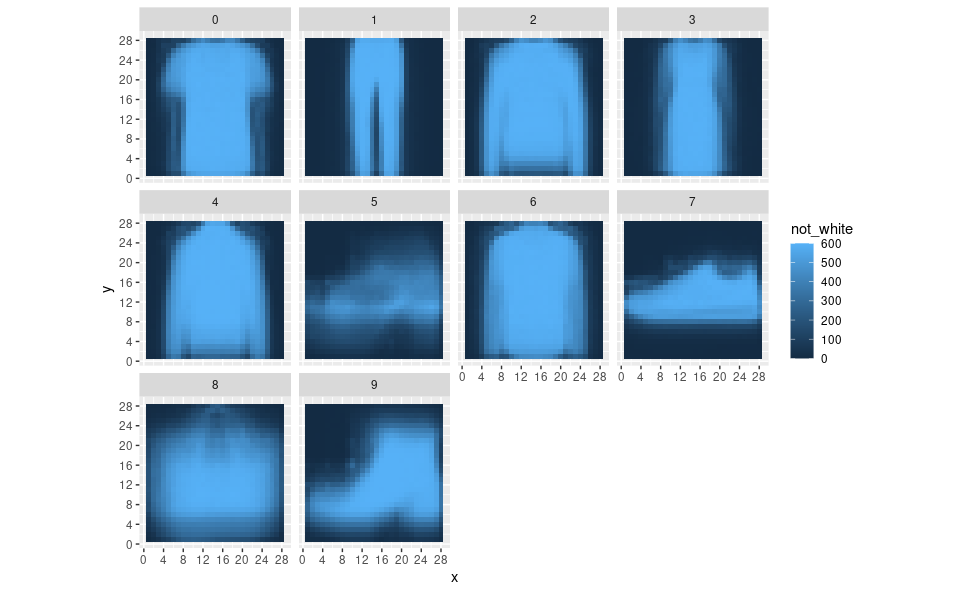
\includegraphics[width=0.9\linewidth]{/home/bonzilla/Documents/MSDS/Data622_group5_projects/FinalReport_Data622/ly_catpixused} 

}

\caption{Categorical Heat Map: Each panel shows mean pixel intensity for each Fashion-MNIST category}\label{fig:unnamed-chunk-3}
\end{figure}

Figure 3 is similar to Figure 2, however Figure 3 shows the mean pixels
intensity for each Fashion-MNIST categorical label. Here we are
attempting to generalize the shapes and pixels used by each of the
different fashion items. Looking at the shoes, we can see that there are
full horizontal rows that are completely white, which is also common to
bags. As we look at the differences and similarities of each of the
classes, the shape of different sections allows us to classify the
labels in our minds, which we'll try to replicate with feature
engineering that follows. If we can create new variables to try and
capture the differences in shape, we can see if those variables will be
useful in contributing to the accuracy of the models we train.

Below is a description of the engineered feature set:

\begin{itemize}
\tightlist
\item
  \% of pixels that are different shades of grey -- 0, 50, 87, 167, 209,
  255

  \begin{itemize}
  \tightlist
  \item
    white: 0
  \item
    grey1: 1-46
  \item
    grey2: 47-93
  \item
    grey3: 94-168
  \item
    grey4: 169-205\\
  \item
    black: 206-255
  \end{itemize}
\item
  \% of non-white pixels in each of the 28 rows
\item
  \% of non-white pixels in each of the 28 columns
\item
  \% of rows that are completely white
\item
  \% of columns that are completely white
\item
  10 custom blocks that are subsections of the grids, showing percent
  non-white as well as percent light grey (1 - 122).
\end{itemize}

The features listed were determined by visually analyzing the Figure 3.
Moving forward in this report, this feature set will be referred to as
the Feature Engineered dataset. For detailed code that describes the
feature generation, please refer to the report code documentation.

\hypertarget{modeling-fashion-mnist-with-the-featured-engineered-dataset}{%
\subsection{Modeling Fashion-MNIST with the Featured Engineered
Dataset}\label{modeling-fashion-mnist-with-the-featured-engineered-dataset}}

Once the Feature Engineered dataset was generated, we performed 10 fold
cross validation to train the following models:

\begin{itemize}
\tightlist
\item
  Random forest
\item
  Support vector machine using a radial kernel
\item
  k-Nearest Neightbor
\item
  Multinomial logistic regression
\item
  Naive Bayes
\end{itemize}

These models were trained exclusively on our Feature Engineered dataset.
Additionally, in order to deal with the hardware limitations of personal
computers, the training data will only use a fraction of the original
60,000 training records. The training set used was a stratified sample
which accounts for 16.7\% or 10,010 observations of the original
training set.

\begin{table}
 \caption{Model Training Summary}
  \centering
  \begin{tabular}{llll}
    \toprule
    Model Type     & Training Duration (min)  & Training Accuracy & Test Accuracy \\
    \midrule
    SVM (Radial) & 19.0  & 0.854 & 0.856 \\
    Multinomial Log Reg     & 9.3  &  0.861 & 0.824 \\
    Random Forest     & 5.5  &  0.799 & 0.855 \\
    k-NN     & 2.6  &  0.8292 & 0.795 \\    
    Naive Bayes     & 0.2  & 0.715 & 0.713 \\    
    \bottomrule
  \end{tabular}
  \label{tab:table}
\end{table}

Table 1 gives a summary of a few select metrics that describe the
training and evaluating of the different model approaches. In terms of
training duration, the fastest model was Naive-Bayes at 0.2 minutes.
However, the radial Support Vector Machine (SVM) model trained for the
longest at 19 minutes. Model duration is important to consider,
especially since all modeling procedures using the Engineered Feature
dataset we used a subset of \textasciitilde10,000 training instances.
Despite the long training, the radial SVM model performed the best by
scoring the highest accuracy on the test data. However, the Random
Forest model achieved a comparable test accuracy. Therefore, if a long
training durations are of concern, the Ransom Forest model is a
reasonable alternative.

\begin{figure}

{\centering 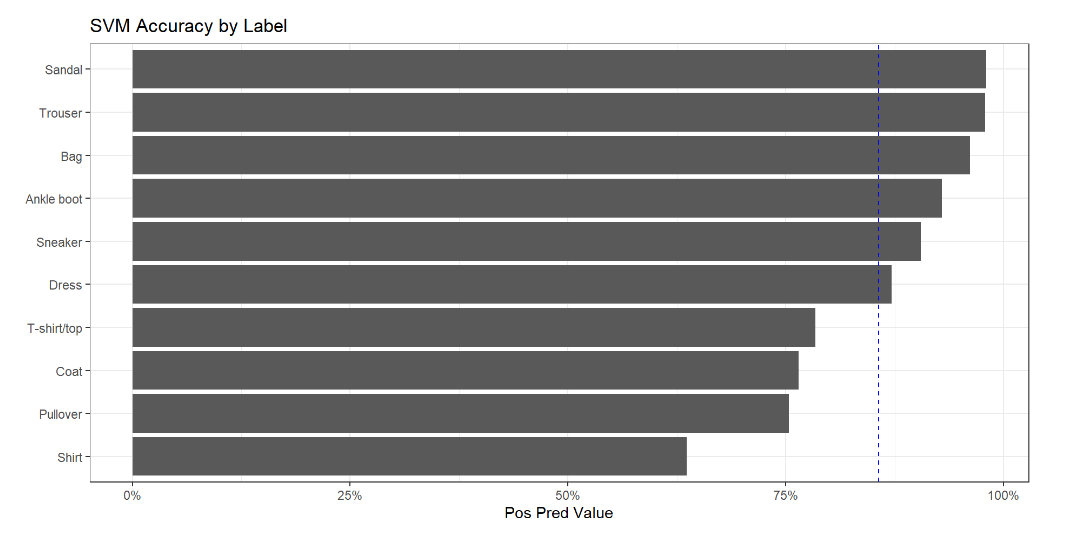
\includegraphics[width=0.9\linewidth]{/home/bonzilla/Documents/MSDS/Data622_group5_projects/FinalReport_Data622/ly_SVMlabelacc} 

}

\caption{SVM Accuracy by Label. the accuracy for each Fashion-MNIST label category is given as a row in this vertical bar chart. The blue line shows the overall accuracy for classification of the test data.}\label{fig:unnamed-chunk-4}
\end{figure}

The performance accuracy given in Table 1 is an important measure of a
model's performance. However, it is not a very thorough measure of a
model's ability to predict the proper labels. Therefore, we also looked
at accuracy for the SVM model broken down by category. Figure 4 shows
the accuracy for each Fashion-MNIST categorical label. As expected, the
errors for the SVM model trained using only variables summarizing
subsections or shapes of the original training data led to specific
items of clothing to be confused for others. For instance, similarly
shaped items such as `Shirt,' `Pullover,' and `Coat' show the lowest
accuracy for classifications. The similar shapes of the items suggest
that the derived variables that were used did not adequately pick up the
variance among the items. Furthermore, the confusion matrix for the SVM
model (see report code documentation) show common misclassifications of
pullovers as coats and shirts as t-shirts/tops or pullovers.
Additionally, for each of the three types of footwear, the errors
predicted by the model are most likely one of other two footwear types.

\hypertarget{modeling-fashion-mnist-with-principal-component-analysis}{%
\section{Modeling Fashion-MNIST with Principal Component
Analysis}\label{modeling-fashion-mnist-with-principal-component-analysis}}

\hypertarget{principal-component-analysis-of-fashion-mnist}{%
\subsection{Principal Component Analysis of
Fashion-MNIST}\label{principal-component-analysis-of-fashion-mnist}}

\label{sec:headings}

We have shown above that there is redundancy in the fashion MNIST
dataset. Here we will use PCA to reduce the number of features while
retaining as much of the variance possible. PCA does this by finding a
new set of axes that fit to the variance of the data. At heart, PCA is
simply an eigendecomposition of the data which returns a set of
eigenvectors and eigenvalues. Eigenvectors and eigenvalues describe the
transformations necessary to go from the original axes to a new feature
space.

We can use the results of PCA to perform a type of information
compression on the original data by subsetting the amount of PCA
components we use to describe the original data. For this analysis, we
will use a criterion of 95\% variance explained. From the 784 components
that PCA yields, we will subset the minimum components needed such that
the sum of the proportions of explained variance is greater than or
equal to 95\%. Such a manipulation is favorable because it will reduce
redundancy in the data, the chances of overfitting, and the time
necessary to train models.

\begin{figure}

{\centering 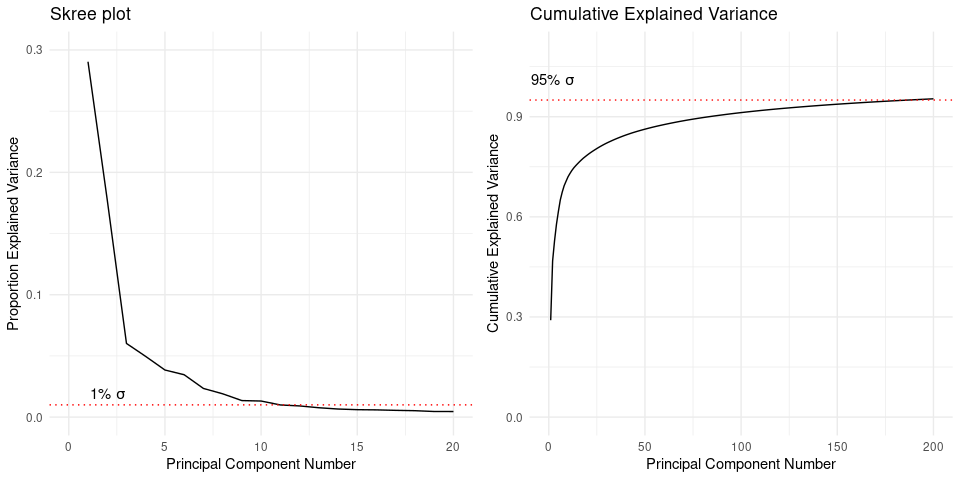
\includegraphics[width=0.9\linewidth]{/home/bonzilla/Documents/MSDS/Data622_group5_projects/FinalReport_Data622/pcaskree} 

}

\caption{PCA Results. The Skree plot (Left) shows the proportion on explained variance for each the first 20 principal components. The Cumulative Explained Variance plot (Right) shows the total variance explained by successively addding up to 200 principal components}\label{fig:unnamed-chunk-5}
\end{figure}

From the skree plot, we can see a very sharp drop off in the proportion
of explained variance. Principal Components greater than 12 account for
less than 1\% of the dataset's variance. The first 12 components only
account for a cumulative variance of 0.74, therefore it takes the
combined contribution of many more components (187 components) to
explain 95\% of the variance of each pixel for the original images.

\begin{figure}

{\centering 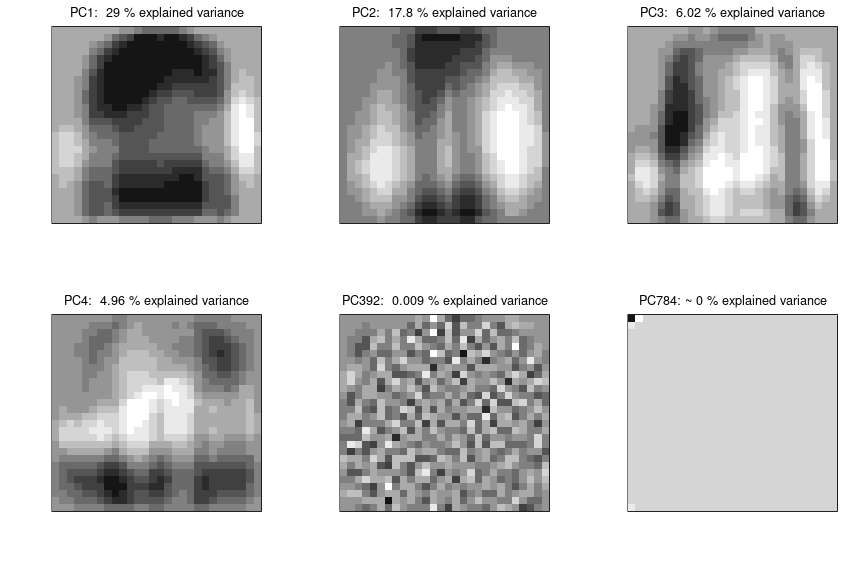
\includegraphics[width=0.9\linewidth]{/home/bonzilla/Documents/MSDS/Data622_group5_projects/FinalReport_Data622/pcacomps} 

}

\caption{Visualizing PCA Components. The top row (from left to right) and bottom left panel visualize principal components 1 through 4. The middle panel of the bottom row shows the 392th component. The bottom right panels shows principal component 784}\label{fig:unnamed-chunk-6}
\end{figure}

PCA returns a components for every dimension of the data in descending
order of the amount of variance accounted for. The figure above shows
the the first 4 components, component PC392 (middle), and the last
component PC784. As already depicted in the Skree and Cumulative
Explained Variance plots, the first four components explain 0.58\%
variance from PC1: 22.1\% \(\rightarrow\) PC2: 5.1\% variance. We can
see clearly from the visualization of the components that the first
several PCs are clearly discriminating between clothing classifications.
For instance, PC1 distinguishes between T-shirt/top \& Pullover
(dark/high values) and shoe categories (light/low values). On the other
hand, PC2 appears to distinguish Trousers from shoe categories. The
representation become less clear as the explained variance decreases.
For instance, PC392 and PC784 only explain 0.01\% and 0.001\% variance
respectively and it is not clear from the visualization just what
information these components represent.

PC1 and PC2 account for roughly half (0.47) of the train dataset's
variance. We can visualize the projections of the train data onto the
features space of these two components:

\begin{figure}

{\centering 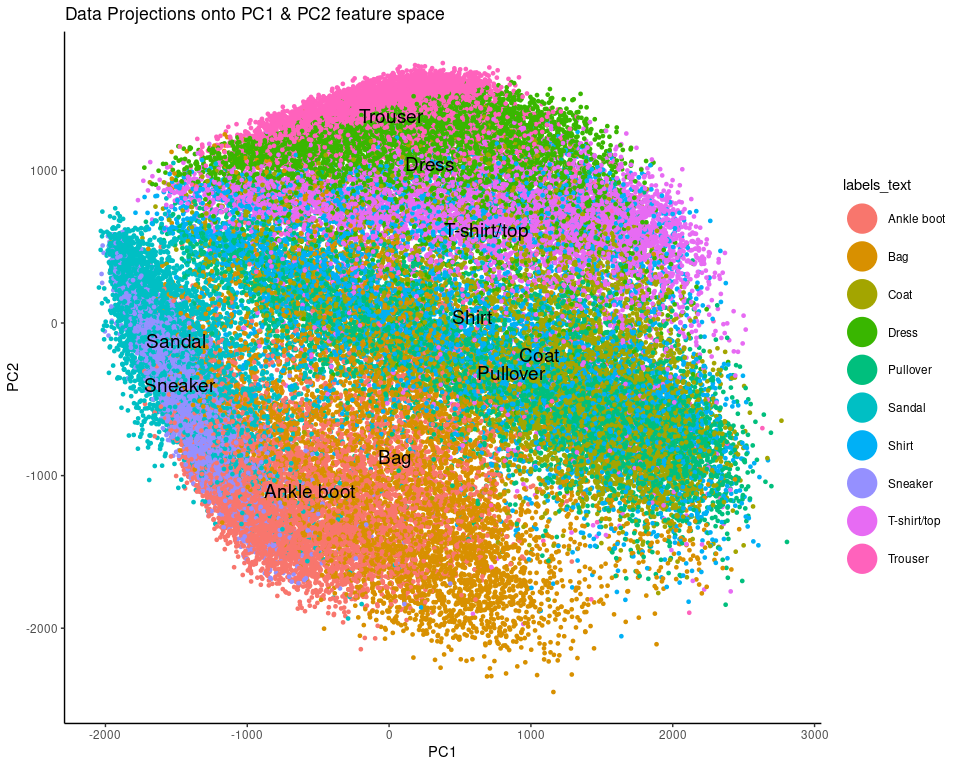
\includegraphics[width=0.9\linewidth]{/home/bonzilla/Documents/MSDS/Data622_group5_projects/FinalReport_Data622/pcaproj} 

}

\caption{Magnitudes of PCA 1 and 2 for all Fashion-MNIST images from the 'train' dataset. Datapoints are shaded according the clothing category. A black text label is rendered at the mean PC1 and PC2 values for each category.}\label{fig:unnamed-chunk-7}
\end{figure}

The figure above shows the representations of the \texttt{train} images
in the feature space of the first 2 dimensions. Each clothing item
category is represented by a different color. For clarity, a text label
(in black) which corresponds to the categorical mean values of PC1 \&
PC2 has been added. We can see that there is noticeable separation
across the categories. Additionally, we see some clustering of category
means that meets expectations. For example, the shoe categories (Sandal,
Sneaker and Ankle Boot) group together towards the lower left hand
corner of the figure. Clothing items that could all be described as tops
with sleeves ( Pullover, Coat, Shirt \& T-shirt/top) group together in
the middle of the distribution. Trousers, on the other hand, have a
noticeable distance from tops with sleeves but ar contiguous with the
dress category which shares roughly vertical rectangular profile.

Here we find the representation onto the first 187 components which were
shown earlier to account for 95\% of the variance in the image data:

\begin{figure}

{\centering 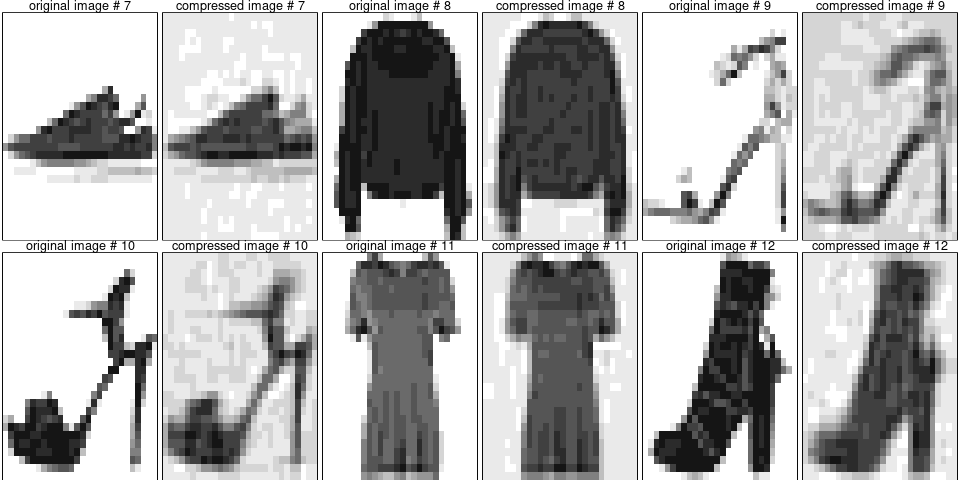
\includegraphics[width=0.9\linewidth]{/home/bonzilla/Documents/MSDS/Data622_group5_projects/FinalReport_Data622/pca_reconstruct} 

}

\caption{Reconstructed Images using 187 Principal Components. Original Fashion-MNIST images are rendered next to the corresponding compressed images which are reconstructed from the first 187 components}\label{fig:unnamed-chunk-8}
\end{figure}

Truncating the data to 187 components does result in information loss,
however, as we can see from the visualizations above, the images retain
much of the detail from the original images while using a feature space
23.85\% the size of the original.

PCA is a dimensionality reduction method that can be applied to high
dimensional datasets. PCA reduces the number of features while
preserving as much variance from the data as possible. Here we used PCA
to reduce the number of features of the Fashion MNIST dataset from 784
to 187. We showed through a series of visualizations that transforming
the images to the reduced feature space does so with an noticeable loss
to image quality, however the gist of the images are still present.

\hypertarget{modeling-fashion-mnist-with-and-without-the-use-of-pca-compression-k-nearest-neighbors-svm}{%
\subsection{Modeling Fashion-MNIST with and without the use of PCA
Compression: k-Nearest Neighbors \&
SVM}\label{modeling-fashion-mnist-with-and-without-the-use-of-pca-compression-k-nearest-neighbors-svm}}

In the previous section, we showed that PCA can be used on Fashion-MNIST
to reduce the dimensionality of the data to less than \(\frac{1}{4}th\)
the original size. Here we implement Support Vector Machine and
k-Nearest Neighbor, both non-parametric methods, to classify
Fashion-MNIST images using both the original data which uses all 784
columns of pixel values as features and the PCA compressed data which
reduces the feature space the 187 columns. As in other analyses in the
report, these models will also be `trained' on a subset of 10000
samples, both to reduce training times.

K-Nearest Neighbors (kNN) is a non-parametric technique that can be used
for image classification. It's a very simple technique, wherin new
samples are classified as the most typical class among the `k' nearest
labeled examples it was `trained' on where `k' is an integer value. That
being said, kNN doesn't actually train, rather, it stores the data and
refers back to it when making classifications. For our analysis, the
\texttt{caret} package was used to create this model, and although it
may appear like it's fitting a model, what it's actually doing here is
storing all the training data, then trying out different `'k values, one
of which it will choose to use when 'predict' is called. Even if it's
not semantically well implemented, it's still very useful for finding a
good `k' value.

\begin{Shaded}
\begin{Highlighting}[]
\CommentTok{\#Validation accuracy for different values of k }
\CommentTok{\#plot(knn.fit)}
\end{Highlighting}
\end{Shaded}

We begin by fitting a kNN model to the original Fashion-MNIST dataset.
Although this analysis starts with all 784 features, whittle down some
of the data by choosing only variables (pixels) which vary significantly
between images. For example, if a pixel in the corner of the images has
the same value throughout most images, this pixel will dropped from the
data and not be used in fitting model. For full details and code, please
refer to the report code documentation. Figure XXXX shows the
cross-validation accuracies across several values of `k.' This plot give
the hyperparameter tuning curve for the model. We see that k=5 performed
as the best value with the training data.

With k=5, we evaluated the model performance for classifying the test
data. The overall accuracy for this model was 81.33\% (95\% CI: 80.57 -
82.09\%). The confusion matrix (see report code documentation) shows
that the model has an easier time detecting some labels than others. For
example, it correctly classifies most of the sneakers (label 7), bags
(8), ankle-boots (9), and trousers (1). However, it has a much harder
time classifying pullovers (2), coats (4), sandals (5), and shirts (6).
Shirts in particular fared poorly, with only about half correctly
classified; t-shirts/tops (0), pullovers (2), and coats (4) were also
often missclassified as shirts, which makes sense (they are very
similar).

PCA kNN Now we'll try kNN with the PCA compressed data, and see if it
has any effect on performance when compared to the previous model. When
`fit' on a sample of 10,000 samples, a k value of 7 appears to perform
best during cross-validation. The cross-validation accuracies across k
values of 1-11 were similar; below, this is plotted.

\begin{Shaded}
\begin{Highlighting}[]
\CommentTok{\# plot(knn.pca.fit)}
\end{Highlighting}
\end{Shaded}

The changes in accuracy avross different values of k (above) aren't
terribly drastic. K values of 5-7 performed best across all tested
values (not all included above).\\
Let's try it out on the test set now. The overall accuracy of this model
was 82.36\% (95\% CI: 81.61 - 83.11\%). It performed very similarly to
the previous model which used a non-pca compressed dataset. We can see
similar patterns in the confusion matrix:most of the sneakers (label 7),
bags (8), ankle-boots (9), and trousers (1) where correctly classified.
Also, it had a harder time classifying pullovers (2), coats (4), sandals
(5), and shirts (6). We also see similar missclasifications to the other
set, where shirt classification is poo, and t-shirts/tops (0), pullovers
(2), and coats (4) were often missclassified as shirts. Similar to wat
we saw with the SVM models, the PCA compressed kNN model actually
performs slightly better than the regular kNN model (82.35\% vs 81.23\%
overall accuracy; a significant difference at \(\alpha = 0.05\)). It's
unclear why this happens. One could theorize that perhaps the removing
some of the percision in the data may make for more robust models that
resist over-fitting. It could also be seperating the data a bit better,
which both SVM and kNN would benefit from significanly.

\hypertarget{modeling-fashion-mnist-using-pca-compression-additional-machine-learning-models}{%
\subsection{Modeling Fashion-MNIST using PCA Compression: Additional
Machine Learning
Models}\label{modeling-fashion-mnist-using-pca-compression-additional-machine-learning-models}}

PCA is a dimensionality reduction method that can be applied to high
dimensional datasets. PCA reduces the number of features while
preserving as much variance from the data as possible. Here we used PCA
to reduce the number of features of the Fashion MNIST dataset from 784
to 187. We showed through a series of visualizations that transforming
the images to the reduced feature space does so with an noticeable loss
to image quality, however the gist of the images is still present.
Furthermore, we used SVM model fits to evaluate performance with the
reduced dimension PCA version of Fashion MNIST. A radial SVM classifier
was trained on a subset of 10,000 images for both the full-featured set
and the PCA-compressed set. The PCA-compressed model trained
approximately 1 minute and 20seconds faster than the full-featured data.
En face, this does difference does not sound appreciable. However,
considering that training time for SVM scales quadratically with dataset
size, one would expect to see noticeable improvements in performance had
the entire \texttt{train} set been used for model training. Furthermore,
we evaluated the classification accuracy and found that the
PCA-compressed SVM model had a higher prediction accuracy on the test
data. In conclusion, use of the PCA compressed dataset would be
beneficial in down-stream modeling analysis. As a detraction, additional
steps would be necessary to transform the data between full and
compressed feature spaces to facilitate model interpretation.

\hypertarget{report-directions}{%
\section{Report Directions}\label{report-directions}}

In your report, be sure to:

\begin{itemize}
\item
  describe the problem you are trying to solve.
\item
  describe your datasets and what you did to prepare the data for
  analysis.
\item
  methodologies you used for analyzing the data
\item
  why you did what you did
\item
  make your conclusions from your analysis. Please be sure to address
  the business impact (it could be of any domain) of your solution.
\end{itemize}

\hypertarget{refs}{}
\begin{CSLReferences}{1}{0}
\leavevmode\hypertarget{ref-krizhevsky2009learning}{}%
Krizhevsky, Alex, Geoffrey Hinton, and others. 2009. {``Learning
Multiple Layers of Features from Tiny Images.''}

\leavevmode\hypertarget{ref-lecun1998gradient}{}%
LeCun, Yann, Léon Bottou, Yoshua Bengio, and Patrick Haffner. 1998.
{``Gradient-Based Learning Applied to Document Recognition.''}
\emph{Proceedings of the IEEE} 86 (11): 2278--2324.

\leavevmode\hypertarget{ref-noever2021overhead}{}%
Noever, David, and Samantha E Miller Noever. 2021. {``Overhead Mnist: A
Benchmark Satellite Dataset.''} \emph{arXiv Preprint arXiv:2102.04266}.

\leavevmode\hypertarget{ref-xiao2017fashion}{}%
Xiao, Han, Kashif Rasul, and Roland Vollgraf. 2017. {``Fashion-Mnist: A
Novel Image Dataset for Benchmarking Machine Learning Algorithms.''}
\emph{arXiv Preprint arXiv:1708.07747}.

\end{CSLReferences}

\bibliographystyle{unsrt}
\bibliography{references.bib}


\end{document}
